% !TEX encoding = UTF-8 Unicode

\documentclass[a4paper]{article}

\usepackage{color}
\usepackage{url}
\usepackage[T2A]{fontenc} % enable Cyrillic fonts
\usepackage[utf8]{inputenc} % make weird characters work
\usepackage{graphicx}
\graphicspath{{slike/}}
\usepackage{amssymb}
\newcommand*{\field}[1]{\mathbb{#1}} % Set of Real numbers
\usepackage{amsmath}

\usepackage[english,serbian]{babel}
%\usepackage[english,serbianc]{babel} %ukljuciti babel sa ovim opcijama, umesto gornjim, ukoliko se koristi cirilica

\usepackage[unicode]{hyperref}
\hypersetup{colorlinks,citecolor=green,filecolor=green,linkcolor=blue,urlcolor=blue}

%\newtheorem{primer}{Пример}[section] %ćirilični primer
\newtheorem{primer}{Primer}[section]

\begin{document}

\title{Unija intervala na realnoj pravoj, \\ Can we do better? \\  \small{Seminarski rad u okviru kursa\\Konstrukcija i analiza algoritama 2\\ Matematički fakultet}}

\author{Milan Čugurović, 1009/2018\\ milan\_cugurovic@matf.bg.ac.rs}
\maketitle

\abstract{
Tema ovog seminarskog rada jeste novi algoritam resavanja problema u odnosu na onaj koji je inicijalno predstavljen 1977. godine u radu Viktora Klea 'Can the Measure $\bigcup^n [a_i, b_i]$ be Computed in Less than O(n*log(n)) Steps?' \\
Novi pristup pokazuje se efikasniji ako se meri ukupno vreme izvrsavanja, iako i dalje ostaje u istoj asimptotskoj klasi slozenosti.
}

\tableofcontents

\newpage

\section{Opis problema i istorijat}
Problem nalazenja ukupne duzine unije intervala na pravoj pojavio se sedamdesetih godina proslog veka. U smislu algoritmike jedan je od fundamentalnih problema. Rad na ovu temu objavio je vec pomenuti Viktor Kle u radu 'Can the Measure $\bigcup^n [a_i, b_i]$ be Computed in Less than O(n*log(n)) Steps?'\cite{vklee} koji je objavljen aprila 1977. godine u casopisu \textit{The American Mathematical Monthly}, broj 84, na stranama 284 i 285, objavljen od strane Americke matematicke asocijacije. \\

Problem je inicijalno zamisljen tako sto se na ulazu nalazi $n$ intervala $[a_1, b_1]$, $[a_2, b_2]$, ..., $[a_n, b_n]$ na realnoj osi, i ptrebno je naci duzinu njihove unije. U uvodnom pasusu pomenutog rada autor postavlja pitanje na koji nacin je moguce efikasno resiti ovaj problem. Takodje, na istom mestu on predlaze i resenje koje kaze: lista tacaka moze biti sortirana u $O(n*log(n))$ koraka, pa resavanje onda zahteva samo dodatnih $O(n)$ koraka da se prodje kroz ovaj sortirani niz i izracuna duzina unije $\bigcup^n [a_i, b_i]$. \\

Pitanje koje muci autora rada na ovom mestu je to sto ovaj problem, ne zahteva apriori sortiranje koje predstavlja glavnu komponentu slozenosti \cite{vesna} u radu predstavljenog resenja. \\

Ovde se razmatra malo modifikovan problem. Naime, ne samo da se zahteva nalazenje duzine unije intervala, vec se zahteva i generisanje sortianih segmenata koji predstavljaju tu uniju. Na osnovu ovog dodatnoh zahteva, prosiren je i algoritam predstavljen u radu, tako da ima i ovu dodatnu funkcionalnost. \\

\section{Značaj problema}

Pomenuti problem značajan je iz više razloga. Prirodno se pojavljuje u računanju površine datog podskupa euklidske ravni. Naime, pretpostavimo da su $[u_1, v_1]$, $[u_2, v_2]$, ..., $[u_n, v_n]$ dati intervali na realnoj osi, a $f_i$ i $g_i$ neprekidne funkcije na $[u_i, v_i]$, i \begin{equation}
    P_i = \{ (x, y): u_i\leq x \leq v_i, f_i(x) \leq y \leq g_i(x)\}
\end{equation}
Čak i u situacijama kada površine pojedinačnih $P_i$ možemo lako da izračunamo, računanje površine unije $\bigcup_1^n P_i$, ako se $P_i$ seku na netrivijalan način. \\

Međutim, ako su funkcije $f_i$ i $g_i$ Lipšicove (što nije redak slučaj), onda je tražena površina približno jednaka: \begin{equation} \label{fla}
    \sum_{j=1}^n (measure(L_j \cap P))(s_j-s_{j-1}),
\end{equation}
gde je $s_0 < s_1 < ... < s_m$ odgovarajuća dovoljno gusta sekvenca iz $\bigcup_{i=1}^n [u_i, v_i]$ a $L_j$ jeste apscisa $(s_{j-1}+s_j)/2$. Odatle \begin{equation}
    L_j \cap P = \bigcup_{i=1}^n L_j \cap P_i.
\end{equation}

Računanje \ref{fla} uključuje $m$ problema računanja dužne date unije intervala. \\

Drugi praktičan primer neophodnosti modifikovane verzije ovog algoritma jeste slučaj kada nam intervali stižu kontinuirano u određenim diskretnim vremenskim trenutcima. Tada nam je, pored toga sto nam u svakom trenutnu treba dužina unije do sada pristiglih intervala, treba i izlazni niz intervala, da bismo znali šta da činimo sa upravo pristiglim intervalom. U ovome se krije i ideja novog pristupa koji se prezentuje ovim seminarskim radom. 

\section{Rešenja problema}

\subsection{Rešenje iz 1977. godine}

Rešenje prezentovano u referentnom radu iz 1977. godine nužno zahteva sortiranje datih intervala, što predstavlja njegovu osnovnu slabost. Neka su nam dati intervali $[a_i, b_i]$. Pretpostavimo da je svaka početna tačka intervala $a_i$ označena sa 1, dok su krajnje tačke $b_i$ označene sa -1. Koriteći sortiranje koje je loženosti $O(n*log(n))$, niz od ovih $2*n$ tačaka može biti sortiran u rastući redosled $e_1 \leq e_2 \leq ... \leq e_{2n}$ tako da, ako je $t_1, t_2, ..., t_{2n}$ odgovarajuća permutacija oznaka, tada je  je $t_i \geq t_{i+1}$ kada god je $e_i = e_{i+1}$.
Drugim rečima, ako levi i desni krajevi neka dva intervala predstavljaju istu tačku, sortiranjem nikad desni kraj intervala neće doći pre levog kraja. \\

U nastavku je dat pseudokod algoritma koji prvo konstruiše uniju $[c_1, d_1], [c_2, d_2], ..., [c_m, d_m]$ prethodnih intervala $[a_i, b_i]$, a zatim računa dužinu njihove unije. 

\begin{figure}[h!]
\begin{center}
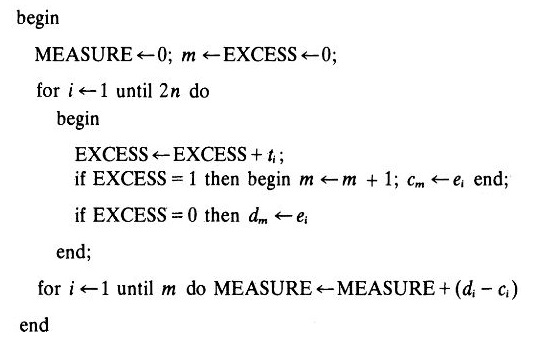
\includegraphics[scale=0.51]{klee_pseudo.JPG}
\end{center}
\caption{Original pseudokod algoritma}
\label{fig:pseudo}
\end{figure} 

Na slici \ref{fig:kleeimp} data je implementacija prethodnog algoritma, sa malim modifikacijama (kod vraća i uniju koju kreira) u programskom jeziku Python. \\

Pomenuta implementacija do detalja prati pseudokod \ref{fig:pseudo} dat u originalnom radu, do na par izmena koje su neophodne radi savladavanja date male modifikacije problema koja se ovde razmatra.

\begin{figure}[h!]
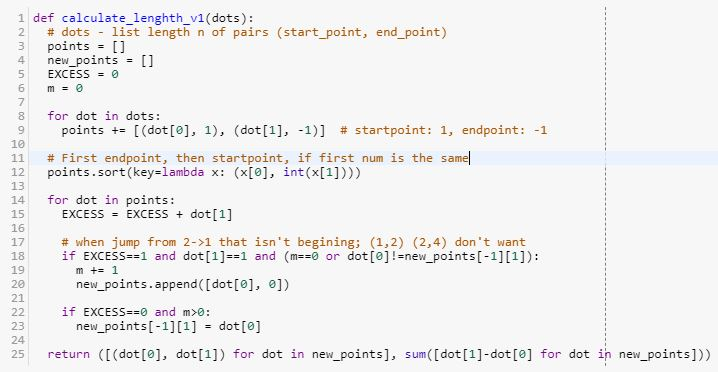
\includegraphics[scale=0.8]{klee_implementacija.JPG}
\caption{Python 3.0 implementacija}
\label{fig:kleeimp}
\end{figure}


\newpage
\subsection{Novi pristup}

Novi pristup zasniva se na sledećoj, veoma jednostavoj ideji. Naime, ideja jeste da se obrađuje interval po interval, dok se u svakom koraku tačno zna. ne samo dužina do sada obraženih intervala, već i njihova unija, kao sortiran niz intervala realne prave. U svakom koraku potrebno je dodatno, za novi pristigli interval pokrenuti dve binarne pretrage kojima se pronalaze mesta levog i desnog kraja novog intervala u vec sortiranoj uniji. Dalje, na osnovu odnosa novih tačaka i dosadašnje unije, preduzimaju se odgovarajuči koraci. \\

Naime, baza indukcije jeste slučaj kada imamo samo jedan interval. Tada je izaz algoritma upravo taj interval, dok je dužin unije u ovom slučaju razlika desnog i levog kraja istog. \\

Indukcijska hipoteza jeste, da za datih $n$ intervala $[a_1, b_1], [a_2, b_2], ..., [a_n, b_n]$ umemo da nadjemo kako dužinu njihove unije $S_n$ tako i sortiranu listu tačaka $[c_1, c_2, ..., c_m]$ gde $c_i$ jeste par $(a_j, True)$ ili $(b_k, False)$ u zavisnosti da li je to kraj ili početak nekog od intervala. \\

Indukcijski korak predstavlja obradu $n+1$-vog intervala $[a_{n+1}, b_{n+1}]$. Prvo se, pokreću dve binrne pretrage koje rade u složenosti $O(log(m))$ i koje pronalaze odgovarajuća mesta tačaka $(a_{n+1}, True)$ i $(b_{n+1}, False)$ u nizu $[c_1, c_2, ..., c_m]$. U zavisnosti od medjusobnog polozaja novih tačaka i tačaka iz niza $c_i$ vrši se eventualno dodavanje tačaka nizu i povećavanje dužine unije intervala $S_{n+1}$ prema sledećim pravilima: 

\begin{figure}[h!]
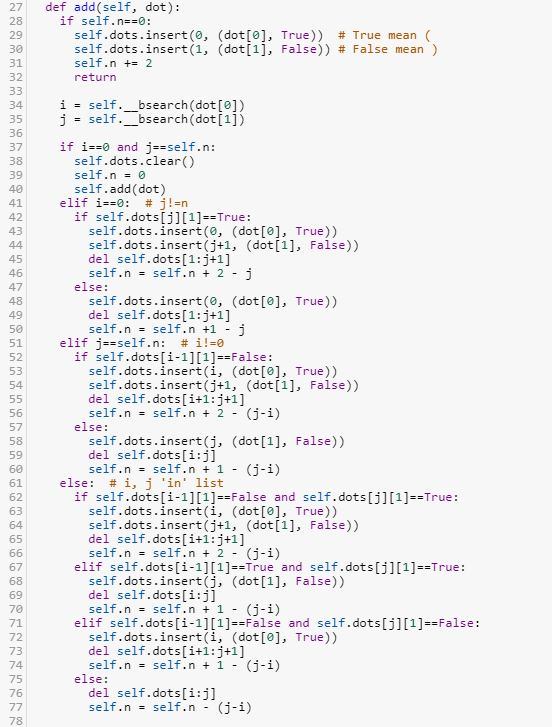
\includegraphics[scale=0.8]{add.JPG}
\caption{Implementacija koraka obrade novog, $n+1$-vog intervala}
\label{fig:add}
\end{figure}

\newpage
Implementacija nove ideje data je kroz implementaciju klase 'Intervaler' ciji se source kod moze naci u pratećim materijalima ovog dokumenta. Klasa implementira prethodni algoritam dodavanja kroz metodu 'add', ali i ostale dodatne neophodne funkcionalnosti.

\section{Implementacija}

\subsection{Specifikacija}

Seminarski rad je implementiran kao Jupyter notebook u programskom jeziku Python, verzija 3.0. \\
Kod je izvršavan na Google colab\cite{gcolab} serveru, čije su specifikacije:
\begin{itemize}
    \item 2 core CPU
    \item each core: Intel(R) Xeon(R) CPU @ 2.30GHz
    \item 13GB RAM
\end{itemize}

Detaljne specifikacije sistema mogu se videti u pratećem notebook kodu.

\subsection{Merenje vremena izvršavanja}

Merenja su vršena nad intervalima koji pripadaju uniformnoj raspodeli na segmentu $[-10, 10]$, pri čemu je i dužina pojedinačnog intervala generisana iz uniformno od 0 do 5. \\ 

Rezultati merenja dati su sa (n predstavlja broj intervala):
\begin{itemize}
    \item $[n = 10]$ originalna ideja: 1.64ms, nova ideja: 643$\mu$s
    \item $[n = 100]$ originalna ideja: 1.8ms, nova ideja: 1.67ms
    \item $[n = 10 000]$ originalna ideja: 37.7ms, nova ideja: 31.3ms
    \item $[n = 1 000 000]$ originalna ideja: 1min 51ms, nova ideja: 25.9s
\end{itemize}

\textbf{Na osnovu prethodnih rezultata zapažamo veoma veliko ubrzanje novog metoda u slučaju dosta gustog \footnote{U smislu kada je broj intervala koji predstavlja disjunktnu uniju ulaza m, dosta manji od broja ulaznih intervala n} skupa intervala.} \\

Dodatno u nastavku je dat grafički prikaz rezultata nekih merenja vremena izvršavanja algoritama. Više informacija nalazi se u pratećem notebook dokumentu.

\begin{figure}[h!]
\begin{center}
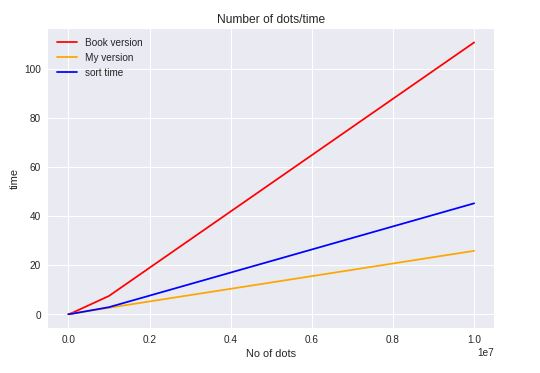
\includegraphics[scale=0.8]{time1.JPG}
\end{center}
\caption{No of dots = $[1, 10, 100, 1000, 10 000, 100 000, 1 000 000, 10 000 000]$}
\label{fig:add}
\end{figure}

\begin{figure}[h!]
\begin{center}
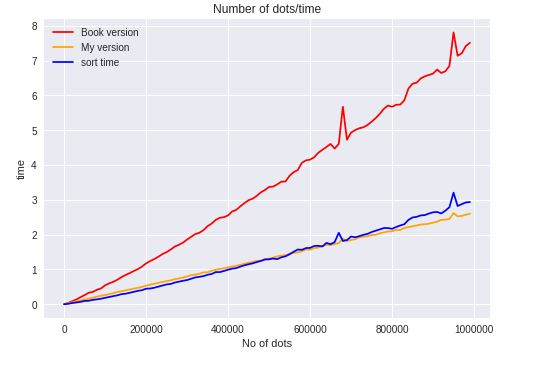
\includegraphics[scale=0.8]{time2.JPG}
\end{center}
\caption{No of dots = $range(10, 1 000 000, 10 000)$}
\label{fig:add}
\end{figure}



%%%%%%%%%%%%%%%%%%%%%%%%%%%%%%%%%%%%%%%%%%%%%%%%%%%%%%%%%%%%%%
\clearpage
\addcontentsline{toc}{section}{Literatura}
\appendix
\bibliography{seminarski} 
\bibliographystyle{plain}

\end{document}
